\section{Grundlagen}
%- Wissenschaftlicher Stand
\subsection{Architektur von Virtual-Reality-Anwendungen}\label{sec:ArchitekturAnwendungen}\todo[inline, color=green]{Lukas}
Bei der Entwicklung von Virtual Reality (VR) Anwendungen gibt es zwei entscheidende Unterschiede im Vergleich zu normalen Software-Anwendungen~\cite{bryson1995approaches}:
\begin{itemize}
	\item die virtuelle Umgebung und das damit verbundene Interface sollten auf die vorliegende Aufgabe zugeschnitten werden und
	\item spezielle Anforderungen an die Performanz der Anwendung müssen erfüllt sein, damit die virtuelle Realität erfolgreich präsentiert werden kann.
\end{itemize}

Als grundsätzlich unterschiedliche Architekturen bei der Entwicklung von Virtual Reality (VR) kann nach Hardware-Plattformen unterschieden werden:
\begin{description}
	\item[Desktop-VR-Applikationen:] hierbei handelt es sich um die leistungsstärksten VR-Applikationen, die potente Computer-Hardware häufig mit Head-Mounted-Displays wie etwa Oculus Rift oder HTC Vive verwenden.
	\item[Mobile-VR-Applikationen:] mobile Anwendungen vereinen häufig (jedoch nicht immer) alle notwendige Hardware in einem Gerät, wie etwa einem Smartphone oder Tablet-Computer.\\ Beispiele für mobile VR-Anwendungen sind Samsung GearVR~\cite{website:gearVRpressRelease} und Google Cardboard~\cite{website:googleCardboard}. Im Falle von Samsung GearVR und Google Cardboard wird zusätzlich eine Haltevorrichtung für das verwendete Gerät eingesetzt, die bei GearVR auch als Controller fungiert und durch ein integriertes Linsensystem das Sichtfeld des Benutzers erhöht.
	\item[Web-VR-Applikationen:] Anwendungen für das Web wie etwa WebVR~\cite{website:webVR} erlauben den Zugriff auf Virtual-Reality-Geräte wie Head-Mounted-Displays durch einen Browser. Auf diese Weise können Web-Inhalte mit VR-Hardware konsumiert werden.
\end{description}

Die Entscheidung, für das vorliegende Projekt auf eine Desktop-VR-Anwendung zu setzen, wurde getroffen, weil mobile und Web-VR-Applikationen die folgenden, vom Projektteam als unverzichtbar eingestuften, Voraussetzungen nicht erfüllen konnten.
\begin{itemize}
	\item Es sollte möglich sein, die in \ref{sec:HandtrackingAnwendungen} beschriebenen Handtracking Interaktionsmethoden für die Verwendung von haptischen Würfel-Markern zu verwenden.
	\item Außerdem sollte die verwendete Architektur ein zuverlässiges Echtzeit-Tracking mit geringer Latenz von mindestens einem Dutzend Markern erlauben, wie es in \ref{sec:MarkerTracking} beschrieben wird.
	\item Und schließlich sollte \emph{MArC} die Basis bereitstellen, um später auch mit mehreren Benutzern verwendet werden zu können.
\end{itemize}

\subsection{Haptische Interaktionsmethoden in VR Umgebungen}\label{sec:HaptikAnwendungen}\todo[inline]{Laura}
\subsection{Handtracking Interaktionsmethoden}\label{sec:HandtrackingAnwendungen}\todo[inline]{Paul}
\subsection{Menüführung in VR Umgebungen}\label{sec:MenüAnwendungen}\todo[inline]{Lukas}
\subsection{Netzwerkverbindung anhand ISO/OSI-7-Schichtenmodell}\label{sec:Netzwerk}\todo[inline, color=green]{Laura}

Um die Kommunikation zwischen unterschiedlichsten technischen Systemen zu ermöglichen und zu vereinheitlichen dient das \textit{ISO/OSI-7-Schichtenmodell} \cite{ITU}, welches in Tabelle~\ref{tab:Schichtenmodell} schematisch dargestellt ist. Um die Weiterentwicklung von Kommunikationsmodellen möglichst barrierefrei zu gestalten, sind in dem Modell sieben aufeinanderfolgende Schichten definiert worden, die für einen klar eingegrenzten Teilbereich der Kommunikation zuständig sind. Die Netzprotokolle, die in einer Schicht zum Einsatz kommen, müssen einheitliche Schnittstellen aufweisen, um einen reibungslosen Austausch zu gewährleisten. Entsprechende Beispiele sind der rechten Spalte von Tabelle~\ref{tab:Schichtenmodell} zu entnehmen.\\

\begin{table}
	\centering
	\renewcommand{\arraystretch}{1.4}
	\begin{tabular}{|c|c|c|}
		\hline
		\Absatzbox{}
		\textbf{Nr.} & \textbf{Schicht}&\textbf{Beispiel}\\
		\hline
		7 & Anwendung &  HTTP, SMTP, FTP, DNS\\
		\hline
		6 & Darstellung & HTTP, SMTP, FTP, NNTP, NetBIOS\\
		\hline
		5 & Sitzung& HTTP, SMTP, FTP, NNTP, NetBIOS, TFTP\\
		\hline
		4 & Transport & TCP, UDP, SPX, NetBEUI\\
		\hline
		3 & Vermittlung& IP IPX\\
		\hline
		2 & Sicherung & Ethernet, ATM, FDDI, TR\\
		\hline
		1 & Bitübertragung & Manchester, 10B5T, Trellis\\
		\hline
	\end{tabular}
	\caption{ISO-/OSI-7-Schichtenmodell}
	\label{tab:Schichtenmodell}
\end{table}

Während die Schichten 1-4 als transportorientierte Schichten einzustufen sind, können die verbleibenden Schichten 5-7 als anwendungsorientiert angesehen werden. Da der Austausch von Daten für die Umsetzung von \textit{MaRC} im Vordergrund steht, wird im Folgenden besonders auf die vierte Schicht eingegangen. Dabei werden die beiden Übertragungsprotokolle \textit{Transmission Control Protocol} (TCP) und \textit{User Datagram Protocol} (UDP) vorgestellt. Auf die Aufführung weiterer Übertragungsprotokolle wird bewusst verzichtet, da wie in Kapitel~\ref{sec:Winsock} beschrieben ist, die \textit{Winsock} API die Übertragung über diese beiden Protokolle ermöglicht.s\\
Die Transportschicht stellt eine logische Ende-zu-Ende-Verbindungen dar und dient als Bindeglied zwischen den transportorientierten und anwendungsorientierten Schichten \cite{ITU}.

\begin{description}
\item[TCP:] Dieses Transportprotokoll ist verbindungsorientiert und paketvermittelt. Genaue Details können in dem Standard RFC 793 \citep{rfc793} von 1981 in Erfahrung gebracht werden.

\item[UDP:] Dieses Transportprotokoll wurde aus der Notwendigkeit heraus entwickelt, für die Übertragung von Sprache auf ein, im Gegensatz zur TCP, simpleres Protokoll zurückgreifen zu können. Genaue Details können in dem Standard RFC 768 \citep{rfc768} von 1981 in Erfahrung gebracht werden.
\end{description}

Ein wichtiger Unterschied zwischen den beiden Transportprotokollen ist, dass die Übertragung per TCP im Vergleich zu UDP sicherstellt, dass gesendete Daten korrekt übertragen und empfangen werden. \textcolor{red}{QUELLE??} Dies geschieht dadurch, dass in einem TCP-Socket-Netzwerk Fehlererkennungs- und Korrekturmechanismen enthalten sind, die fehlerhafte Übertragungen der darunterliegenden Internet Protocol (IP) Schicht ausgleichen, also entweder korrigieren oder dafür sorgen, dass fehlerhafte Daten erneut übertragen werden.


\subsection{Bedienkonzepte in VR-Umgebungen}\label{sec:MenüAnwendungen}\todo[inline, color=yellow]{Lukas}
Die Bedienung eines Systems~--~vor allem Dateneingabe und Objektmanipulation~--~in einer Virtual Reality (VR) Umgebung unterscheidet sich stark von der konventionellen Bedienung mit Maus und Tastatur \cite{chu1997multi}. Das Hauptziel einer VR-Umgebung ist Immersion, also das "`Eintauchen"' des Benutzers in die virtuelle Welt. Ein Teil zur Erreichung dieses Ziels sind Methoden, mit denen der Benutzer mit der virtuellen Welt~--~möglichst intuitiv~--~interagieren kann.

\subsection{Green-Keying}\label{sec:Green-Keying}\todo[inline]{Vera}
\subsection{Marker Tracking} \label{sec:MarkerTracking}\todo[inline]{Vera}
In einer VR oder AR Umgebung ist zur interaktiven Positionierung eines 3D Objektes die präzise Bestimmung der Orientierung und Position im 3D-Zielraum notwendig. Zur Lösung dieses Problems muss zunächst ein physisches Objekt in der realen Welt erkannt, zugeordnet und verfolgt werden. Demzufolge ist es notwendig dieses physische Objekt mit einer Videokamera auf zu nehmen. In den resultierenden Bildsequenzen werden die physischen Objekte anhand von festgelegten Merkmalen erkannt. Diese Merkmale können sowohl natürlicher Art sein oder in Form von künstlich erstellten Codes definiert sein. Ein Objekttracking mit natürlichen Merkmalen wird in der Literatur auch als \textit{Markerless Tracking} bezeichnet, während die Verwendung von Codes, beziehungsweise Bildmarken, als \textit{Markerbased Tracking} bekannt ist.

Natürliche Merkmale zur Identifizierung der Objekte sind Textureigenschaften, Kanteninformationen oder bekannte Keypoints. Eine der robustesten und simpelsten Methoden ist die Verwendung von Keypoints \cite{article:MarkerLessBarandiaran2010}\cite{article:MarkerLessWagner:}\cite{article:MarkerLessComport}\cite{article:MarkerLessLowe}, die sowohl in der Ausgangs- als auch in der Kamerawelt bekannt sind. Diese werden mit Hilfe einer Homographie zur Übereinstimmung gebracht. Daraus resultiert die notwendige Transformation zwischen den Welten (siehe Kapitel \ref{sec:calib}). Ein bedeutender Nachteil der Verwendung von Keypoint oder Texturbasierten Verfahren ist, dass sie nur für Objekte mit einem hohen Grad an Texturmerkmalen und Gradientenbeträgen geeignet sind. Aus diesem Grund wurden auch Verfahren \cite{article:MarkerLessStrucktHinterstoisser}\cite{article:MarkerLessStrucktDamen}\cite{article:MarkerLessStrucktPark} entwicklet die sich speziell für texturarme Objekte eignen, wie etwa die in \textit{MArC} verwendeten grünen Rechtecken der Würfel Marker (siehe Kapitel \ref{sec:WürfelMarker}). Andere Autoren verwenden sehr rechenintensive Kantenerkennungsalgorithmen, wie den \textit{Moving Edges Algorithm} \cite{article:MarkerLessEdgeMarchand}. Eine weitere Weiterentwicklung der Kantenbasierten Methoden ist das Modelbased Tracking bei dem die detektierten Kanten eines möglichen Kandidaten mit den 3D-Kantenmodellen des zu verfolgenden Objektes abgeglichen wird \cite{article:MarkerLessModellVacchetti}\cite{article:MarkerLessEdgeAlvarez}\cite{article:MarkerLessEdgeWu}\cite{article:MarkerLessBlasko}.

Im Gegensatz zu dem Markerbased Tracking benötigt diese Art des Trackings keine Veränderung der realen Welt und die Parameter, welche den Tracking-Algorithmus beeinflussen können nicht ohne weiteres kontrolliert werden \cite{article:MarkerLessBarandiaran2010}. Dennoch ist die markerbasierte Detektierung von Objekten sehr rechenaufwändig und eine eindeutige Zuordnung beziehungsweise Identifikation von ähnlichen oder gleichförmigen Objekten, wie den Würfel Marker (siehe Kapitel \ref{sec:WürfelMarker}) ist sehr aufwändig und nahezu unmöglich. Aus diesem Grund ist es für ein System wie \textit{MArC} zum derzeitigem Zeitpunkt sinnvoller die Marker mit codebasierten Markern zu erweitern, die auch nach längerer Verdeckung eine eindeutige Zuordnung von Würfel Marker ermöglichen. In Abbildung \ref{fig:BinMarker} sind vielfältige Beispiele von binären Codes zu sehen, die zum Marker Tracking verwendet werden. Für \textit{MArC} sind vor allem rechteckige binäre Muster vorteilhaft, da aus dem äußeren vier Ecken direkt die Orientierung des Würfel Markers im Raum berechnet werden kann. Während der Inhalt des Muster zur eindeutigen Identifizierung des Würfels beiträgt. 

Bekannte markerbasierte Verfahren mit rechteckigen binären Mustern sind \textit{QR}, \textit{ARToolKit}\cite{article:MarkerARTOOL}, \textit{ARToolKit Plus}\cite{article:MarkerARTOOL2}, \textit{ARTag} \cite{article:MarkerARTag}, \textit{BinARyID}\cite{article:MarkerBinAR} und \textit{ArUco}\cite{article:Aruco2014}. Wie in Abbildung \ref{fig:BinMarker} zu sehen ist, sind bis auf \textit{BinARyID} und \textit{ArUco} alle Muster sehr detailreich und komplex. Diese Eigenschaft ist auf die höhere Bitgröße der Codes zurückzuführen macht die Erkennung in Aufnahmen mit leichter bis starker Bewegungsunschärfe ungleich schwerer und es kommt zu häufiger zu Fehlinterpretationen und Ausfällen. Gerade in einem System wie \textit{MArC} tritt Bewegungsunschärfe sehr häufig aus, wenn die Würfel Marker verschoben werden. Aus diesem Grund eigen sich hier vor allem Muster mit geringer Bitanzahl und einfacheren Mustern, wie zum Beispiel \textit{ArUco}. Diese Marker Bibliothek ist ein \textit{OpenCV} Modul (siehe Kapitel \ref{sec:OpenCV}), welche alle notwendigen Funktionalitäten und Ressourcen für das Tracking und die Orientierungsbestimmung enthält. Ein großer Vorteil dieser Bibliothek ist, dass die Bitgröße und die maximale Anzahl der Identitäten explizit ausgewählt werden kann.


%Zur eindeutigen Identifizierung von den Codes sind vielfältige Schritte notwendig. Zunächst muss das Muster innerhalb eines Bildes oder Videos erkannt, geortet und verifiziert werden. Im Anschluss wird das gültige Muster der entsprechenden Identifikation (ID) zu geordnet sowie die Orientierung des Markers im Kameraraum berechnet. Diese umfangreichen Ermittlungsprozesse werden in der Regel von entsprechenden Bibliotheken zur Verfügung gestellt, wie zum Beispiel das \textit{ArUco} Modul (siehe Kapitel \ref{sec:aruco}) aus dem Bildverarbeitungsbibliothek \textit{OpenCV} (siehe Kapitel \ref{sec:OpenCV}). \\
\begin{figure}[H] 
	\center 
	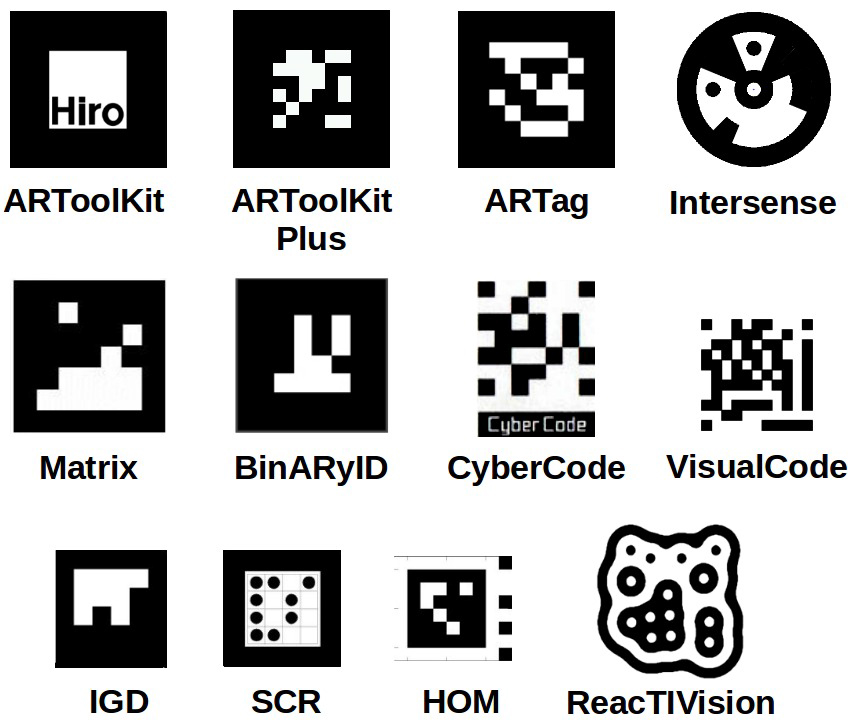
\includegraphics[width=8cm]{Bilder/BinMuster.jpg}			
	\caption{Diverse Binäre Muster die als Code für Markerbasiertes Tracking verwendet werden. Quelle: \cite{article:Aruco2014}}
	\label{fig:BinMarker}
\end{figure}

\newpage